\begin{figure*}[h]
	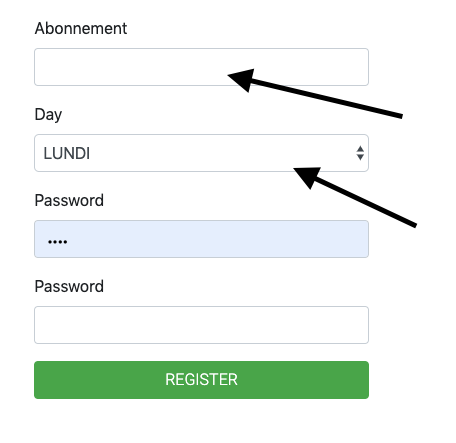
\includegraphics[width=0.5\textwidth,center]{Figures/us4-1}
	\caption{Selection pour l'inscription automatique}
\end{figure*}

\begin{enumerate}
	\item L'utilisateur introduit le nombre de session pour le quelle il paye.
	\item Il selection les sessions pour les quelle il souhaite s'inscrire.
	\item Il clique sur \textit{Register}.
\end{enumerate}

\subsubsection{Gestion des erreurs}
	\paragraph{}
		Si une erreur arrive durant l'inscription l'utilisateur ne sera pas rediriger et aura un message d'erreur. 
	
	
\newpage
\subsubsection{Script concernés}
	\begin{itemize}
		\item \Href{https://github.com/victorsmits/Aquabike/blob/master/backend/src/Controller/RegistrationController.php}{RegistrationController.php}
		\item \Href{https://github.com/victorsmits/Aquabike/blob/master/backend/templates/registration/register.html.twig}{register.html.twig}
		\item \Href{https://github.com/victorsmits/Aquabike/blob/master/backend/src/Entity/Person.php}{Person.php}
		\item \Href{https://github.com/victorsmits/Aquabike/blob/master/backend/src/Entity/Inscription.php}{Inscription.php}
	\end{itemize}
